\documentclass{article}

% Package Pygments for fancy typesetting of code
\usepackage{minted}
\usemintedstyle{default}

\usepackage[T1]{fontenc}
\usepackage[utf8]{inputenc}
\usepackage{color}
\usepackage{graphicx}

% Hyperlinks in PDF: \href{url}{linktext}
\definecolor{linkcolor}{rgb}{0,0,0.4}
\usepackage[%
    colorlinks=true,
    linkcolor=linkcolor,
    urlcolor=linkcolor,
    citecolor=black,
    filecolor=black,
]{hyperref}

\begin{document}

\title{INF3121 \\ Project 1: Interpret the metrics offered by the static analyzer}

\author{
Husein Mehmedagic\footnote{\texttt{huseinm@student.matnat.uio.no}.}
\and
Even Langfeldt Friberg\footnote{\texttt{evenlf@student.matnat.uio.no}.}
}

\date{\today}

% Generate title, author, and date
\maketitle

\renewcommand{\abstractname}{Introduction}
\begin{abstract}
In this project we will make use of one of the authors' first Java code, slightly more than 500 lines, 
which was given as the first mandatory assignment in the course INF1010 taught in spring 2012. The 
original assignment text can be found at \url{http://heim.ifi.uio.no/inf1010/v12/oblig/1/oblig1_.html}.

The GitHub repository for our work can be found at \url{http://github.com/elfriberg/inf3121/tree/master/project1}.
\end{abstract}

\section{Metrics Kiviat Graph on Checkpoint and Significant Other (Step 3)}
\begin{figure}
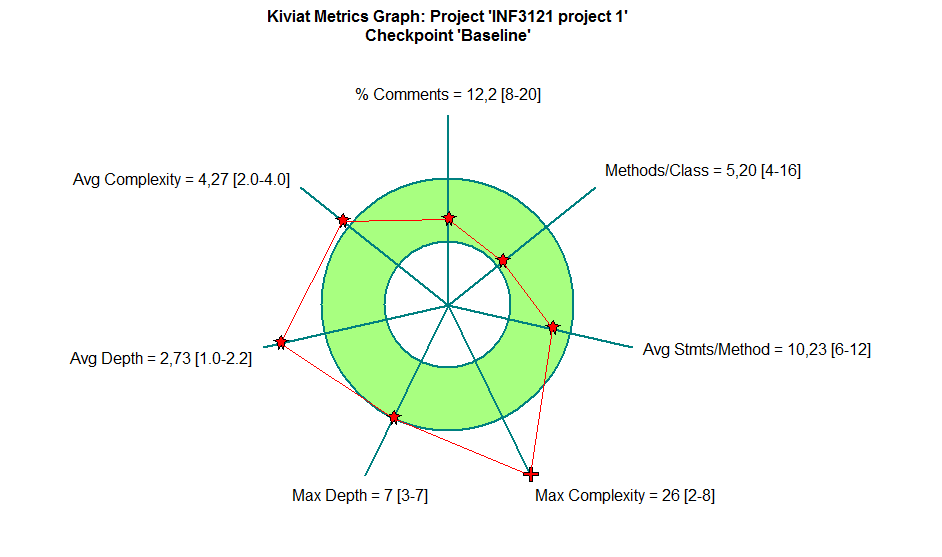
\includegraphics[scale=0.5]{step3-1_kiviat_Baseline}
\caption{
We readily see the complexity and the depth both exceed the boundaries given by the Kiviat graph. Note that this is metrics on all java files in the 
project.
}
\end{figure}

\textit{What does the graph tell you? How do you interpret the metrics applied on your project?}

For the metrics applied on the checkpoint (total project) we observe that although comments are sparse, they are still over a minimum defined by the 
inner boundary. Methods per class says here that this small project follows good object-oriented principles in not overloading a class with too many methods. 
In this case we probably could have done with fewer classes, some of them are very small. Average statements per method seems to be quite okay, within 
boundaries. Max complexity is more interesting: it seems to be 18 points off the outer boundary. Note that this is for one particular method. Considering this is 
the first assignment in an introductory Java subject it is hardly a surprise. The student probably didn't know smarter ways of doing things, and stuck to 
the most basic of structures, and was happy that the code run at all. Note that even though average complexity is on the higher end, it is considerable 
closer to the Kiviat graph than the maximum metric. This means (since there are few lines of code) that there is one (or a few methods) that is much 
more complex than the average.

The depth metric is also outside the outer graph boundary, and it means some methods could have been doing less. If the novice programmer made each method perform 
just a minimum, but ensured that it did what it was supposed to do after he finished it, it might have been easier to debug during development. \\

\noindent We now turn our attention to the two most significant files of the project (\texttt{PersonListe.java}: 197 lines; \texttt{Program.java}: 204 lines) 
and one really small (\texttt{Person.java}: 80 lines). \\

\begin{figure}
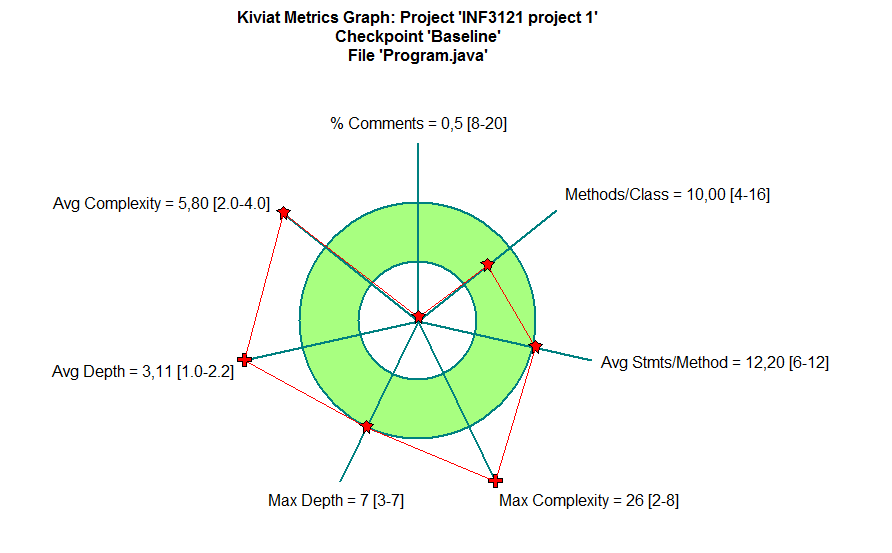
\includegraphics[scale=0.5]{step3-2_kiviat_Program}
\caption{
Kiviat graph for the largest file in the project.
}
\end{figure}

\begin{figure}
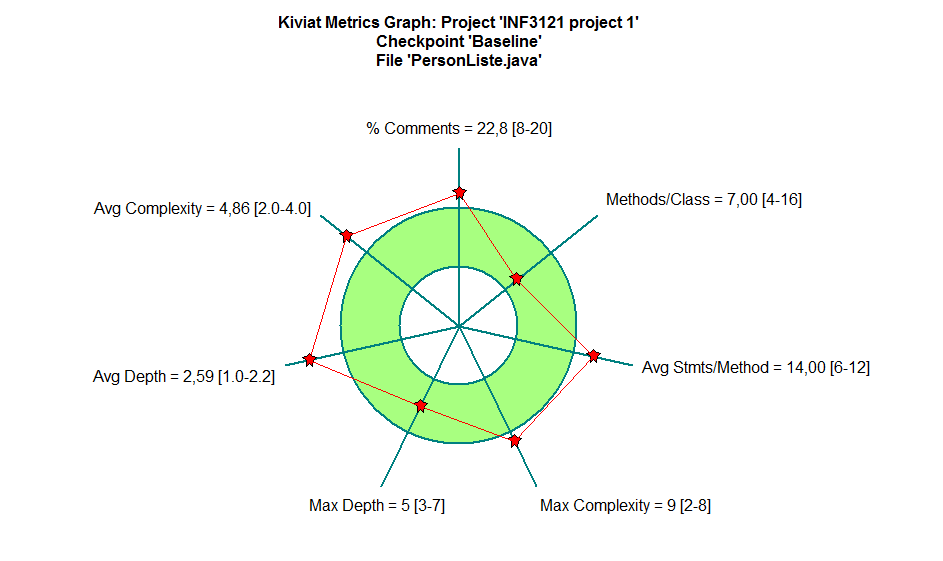
\includegraphics[scale=0.5]{step3-2_kiviat_PersonListe}
\caption{
Kiviat graph for the next-largest file in the project.
}
\end{figure}

\begin{figure}
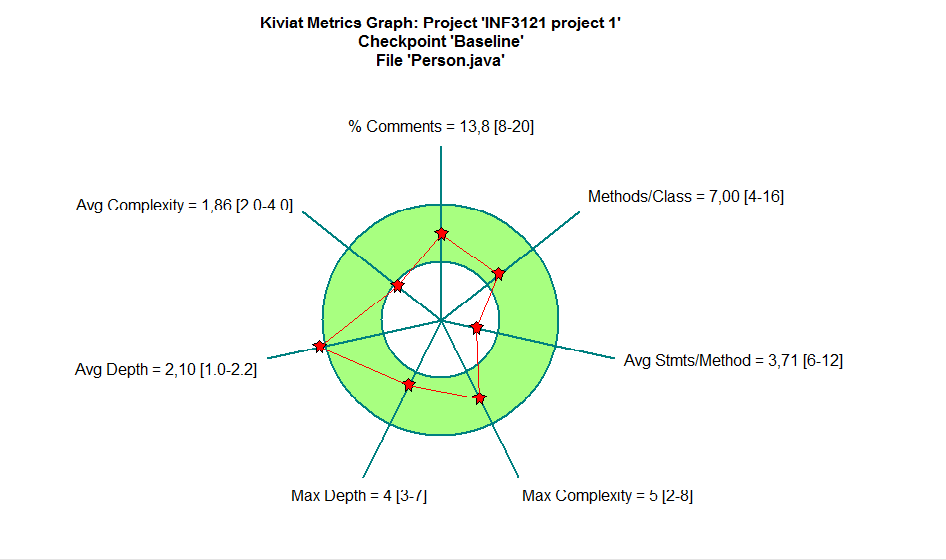
\includegraphics[scale=0.5]{step3-2_kiviat_Person}
\caption{
Kiviat graph for a smaller file in the project.
}
\end{figure}

\textit{What does the graph tell you? How do you interpret the metrics applied on your file? How are they different the metrics you obtained on the whole project, compared with the metrics on this file?}

The Kiviat graph for \texttt{Program.java} helps us identify the family's black sheep. This file consists of virtually no comments. If one can read 
Norwegian this can be excused as the method names make quite a lot of sense. This file contains the code for the terminal user-interface (\texttt{public 
void kommandoProgram}) and commands for e.g. adding a new person (\texttt{public void cmdNyperson}) to the system, a super-simple 'Facebook' system.

Max depth and max complexity is the same as for the checkpoint already considered. Methods per class is well inbetween the limits and average statements 
per method is just on the upper limit.

Offset points from checkpoint:
\begin{enumerate}
 \item Comments: $0.5 - 12.2 = -11.7$
 \item Methods/Class: $10 - 5.2 = 4.8$
 \item Avg Stmts/Class: $12.2 - 10.23 = 1.97$
 \item Max Complexity: $26 - 26 = 0$
 \item Max Depth: $7 - 7 = 0$
 \item Avg Depth: $3.11 - 2.73 = 0.38$
 \item Avg Complexity: $5.8 - 4.27 = 1.53$
\end{enumerate}



\section{Quantative Data (Step 4)}
\textit{What is the biggest file you have in your project? How long the file? How many methods in it?}

\begin{figure}
\centerline{ 
 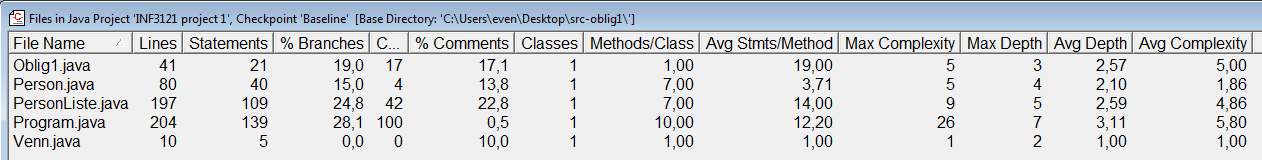
\includegraphics[scale=0.35]{step4}
}
\caption{Step 4}
\end{figure}

The largest file is \texttt{Program.java} consisting of 204 lines (6.9 KB), and 10 methods, including the constructor method. \\

\section{Method Metrics (Step 5)}
\textit{Which is the most complex method in your project? How many statements does it have? - Would you refactor any of the methods you have in your project?
- What can you say about how coupled/decoupled the program is?}

\begin{enumerate}
 \item The most complex method is \texttt{kommandoProgram}, with a complexity of 26. It consists of 40 statements. 
 \item Yes, for sure. \texttt{kommandoProgram} should have been refactored, to get rid of many redundant logical statements. This is also true for 
 \texttt{fjernVenn} who suffers under the linkedlist-structure.
 \item We have 8 methods with more than 10 method-calls. The two most highly-coupled methods make respectively 31 and 17 calls. This is quite a lot 
 for so few lines of code. Changing the structure should be done carefully because several methods are that coupled.
\end{enumerate}


\section{Suggestions for Improvements (Step 6)}
\textit{How would you improve your code, based on the metrics you have obtained with this analyzer?}

\begin{verbatim}
(...)

} else if (innKommando.equalsIgnoreCase("tlf") && (words.length > 2)){
cmdTlf(words[1], words[2]);
} else if (innKommando.equalsIgnoreCase("fjern") && (words.length > 1)){
cmdFjern(words[1]);
} else if (innKommando.equalsIgnoreCase("alle")){
cmdAlle();
} else if (innKommando.equalsIgnoreCase("hjelp")){
cmdHjelp();
} else if (innKommando.equalsIgnoreCase("venner") && (words.length > 2)){
personliste.nyVenn(words[1], words[2]);
} else if (innKommando.equalsIgnoreCase("uvenner") && (words.length > 2)){
personliste.fjernVenn(words[1], words[2]);
} else if (innKommando.equalsIgnoreCase("vis") && (words.length > 1)){
cmdVis (words[1]);
} else if (innKommando.equalsIgnoreCase("tilfil") && (words.length > 1)){
cmdTilfil(words[1]);
} else if (innKommando.equalsIgnoreCase("frafil") && (words.length > 1)){
cmdFrafil(words[1]);
} else if (innKommando.equalsIgnoreCase("slutt")){
System.out.println("Ha det bra!");
}
else {
System.out.println("Kommandoen du gav er ikke på gyldig form");
cmdHjelp();
} 

(...)
\end{verbatim}

This is a snippet of the \texttt{kommandoProgram} method of \texttt{Program.java} with a lot of logical statements. 
We could put all valid command words (i.e. \texttt{hjelp}) in an array, check if the \texttt{innKommando} (or simply 
\texttt{words[0]}) is found in the array, and call the relevant command, or give an error message if the user input a 
typo. Thus we could reduce 10 else-if statements to 1.

\begin{figure}
\centerline{ 
 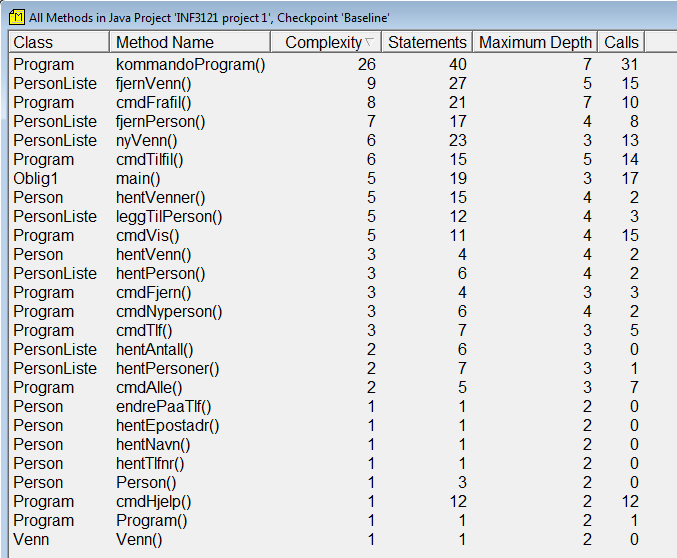
\includegraphics[scale=0.5]{step5_method-metrics}
}
\caption{Step 5}
\end{figure}

\begin{verbatim}
public boolean fjernVenn(String navn, String vnavn){
(...)
else {
  for (Venn peker = a.foersteVenn; peker.nesteVenn != null; peker = peker.nesteVenn) {
    if (peker.nesteVenn.minVenn.hentNavn().equalsIgnoreCase(enVenn.hentNavn())) {
    peker.nesteVenn = peker.nesteVenn.nesteVenn;
    System.out.println("OK: " + vnavn + " er nå fjernet fra vennelisten til " + navn);
    a.venneTeller--;
    return true;
    (...)
\end{verbatim}

This is a snippet of method \texttt{fjernVenn} from \texttt{PersonListe.java}. An objective of this mandatory assignment was to 
implement a self-written LinkedList-structure. The code above could have been much simpler if one made use of the available LinkedList class from 
the Java library (which implements a lot of useful interfaces). 


\end{document}
